\documentclass[a4paper]{article} % A4 paper and 11pt font size

\usepackage{braket}
\usepackage{amsmath}
\usepackage{amssymb}
\usepackage{bm}
\usepackage[utf8]{inputenc}
\usepackage{verbatim}
\usepackage{tikz}
%\usepackage{pgfornament}
\usepackage{pgfplots}
\usepackage{pgffor}
\usepackage[version-1-compatibility]{siunitx}
\usepackage{fancyhdr}
\usepackage{lipsum}
\usepackage{gensymb}
\usepackage{framed}
\usepackage{cancel}
\usepackage{slashed}
\usepackage{hyperref}
\usepackage{pdflscape}
\usepackage{graphicx}
\usepackage{caption}
\usepackage{subcaption}
\usepackage{geometry}
\usepackage{yfonts}
\usepackage{calc}
\usepackage{cite}
\usepackage{siunitx}

\setlength{\parindent}{0em}
\setlength{\parskip}{1em}
\newcommand{\goth}[1]{{\Huge\textfrak{#1}}}
\renewcommand{\baselinestretch}{1.1}

\newcommand{\exercise}[1]
{
\begin{framed}
\textbf{Exercise:} #1 
\end{framed}
}
\newcommand{\example}[2]
{
\begin{framed}
\textbf{Example #1:} #2
\end{framed}
}


 \geometry{
 a4paper,
 total={210mm,297mm},
 left=28mm,
 right=28mm,
 top=30mm,
 bottom=40mm,
 }


%----------------------------------------------------------------------------------------
%	TITLE SECTION
%----------------------------------------------------------------------------------------
%\setlength\parindent{0pt} % Removes all indentation from paragraphs - comment this line for an assignment with lots of text


\pagenumbering{arabic}
\begin{document}
\pagestyle{empty}

\newcommand{\HRule}{\rule{\linewidth}{0.5mm}}

\begin{titlepage}

    \begin{center}
        \textsc{\large SN: 587623}\\[6cm]

        \HRule \\[0.5cm]
		\Huge \textbf{PHYC90012 General Relativity}\\[0.5cm]
        \huge \textbf{Course Summary}\\[0.5cm] 
        \HRule \\[1.5cm]
        \begin{minipage}{0.4\textwidth}
        \begin{center}

        \large By \\[0.75cm]
        \huge Braden \scshape Moore \\[0.5cm]
        \normalsize \normalfont Master of Science \\
        The University of Melbourne \\

        \end{center}
        \end{minipage}

        \vfill

        \large \today
    \end{center}


\newpage
\end{titlepage}
%----------------------------------------------------------------------------------------
\pagestyle{empty}
%\tableofcontents
%\newpage

\pagestyle{fancy}
\pagenumbering{arabic}
\rfoot{\textsc{Braden Moore, 587623}}
\lfoot{\textsc{\today}}
\lhead{\textsc{Semester 1, 2016}}
\rhead{\textsc{PHYC90012 General Relativity}}
\setcounter{page}{1}
\section{Syllabus}
\subsection{Part I}
\begin{enumerate}
\item Introduction to gravity
\begin{itemize}
\item Order of magnitude estimates
\item Small amount of quantum gravity
\end{itemize}
\item Equivalence principle + experimental foundations
\item Geometric objects
\begin{itemize}
\item Need to understand geomtric components of GR
\item Vectors, metric, etc. that live on manifolds
\item Laws of nature do not depend on coordinates chosen
\item Hence can write laws of nature in terms of geometric objects w/o reference to coordinates
\end{itemize}
\item Kinematics
\begin{itemize}
\item Time dilation, length contraction in GR framework
\end{itemize}
\item Calculus in curvilinear coordinates
\begin{itemize}
\item Mass and energy curve spacetime
\item Hence geometric objects moved on curved manifolds
\item Distances are not only spatial but temporal; need to use mathematics of small change = calculus
\item Uses the covariant derivative (a geomtetric object; independent of basis/coordinate independent)
\item This point of the course we will not be considering curved space, but instead only curvilinear coords 
\begin{itemize}
\item A flat space can be covered (represented?) by curved coordinates, but an intrinsically curved surface cannot be covered by flat coordinates
\end{itemize}
\end{itemize}
\item Curved spaces
\begin{itemize}
\item Manifolds 
\item How to calculate lengths, volumes, angles in curved spaces
\item Introduces the idea of parallel transport $\Rightarrow$ leads to curvature
\item Define the Riemann tensor, and its children etc. Ricci tensor, ...; these satisfy the Bianchi identities
\end{itemize}
\item Einsten's field equations
\begin{itemize}
\item Stress-energy tensor
\end{itemize}
\item Weak-field limit
\begin{itemize}
\item Gauge transformations
\end{itemize}
\subsection{Part II - Applications}
\item GR phenomena revisited 
\begin{itemize}
\item GPS, Mercury's orbit, gravitational lensing, gravittional redshift, ...
\end{itemize}
\item Gravitational waves
\begin{itemize}
\item Propagation (phase speed, polarisation, ...)
\item Generation*
\item Detection*
\begin{itemize}
\item * = ``antenna problem"
\end{itemize}
\end{itemize}
\item Relativisitic stars
\begin{itemize}
\item neutron stars
\item equation of state (cannot study on Earth because largest nuclei only have 200 elements or so; need more density)
\end{itemize}
\item Black holes
\begin{itemize}
\item Event horizons, singularities, ...
\end{itemize}
\item Cosmology
\begin{itemize}
\item Friedman-Robertson-Walker (FRW) metric - describes a homogeneous, isotropic universe
\begin{itemize}
\item We will derive this and the Friedman equations
\end{itemize}
\end{itemize}

\end{enumerate}


\section{Introduction to gravity}
\subsection{Strength of gravity}
\begin{itemize}
\item Weak! Weakest of all fundamental forces
\item Long-ranged force (like EM)
\item Weakness determined by coupling constant
\item Coupling constant = Newton's gravitational constant
\end{itemize}
\begin{equation}
\vec{F}=\frac{Gm_1 m_2}{r_{12}^2}\hat{r}
\end{equation}
\begin{itemize}
\item G is hard to measure; least well known of coupling constants
\end{itemize}
In 1797-98, Cavendish used torsion balls (1.8m torsion balance) with rod of big masses and rod of small masses. 
\begin{itemize}
\item Spring constant of torsion balance was measuredfrom free oscillation
\item ten introduced 158kg balls
\item measured delfection angle of balance $\Rightarrow$ force
\begin{itemize}
\item using a mini-telescope against Vernier scale
\end{itemize}
\item rearrange Newton's law to get G
\end{itemize}

\begin{figure}[h]
\centering
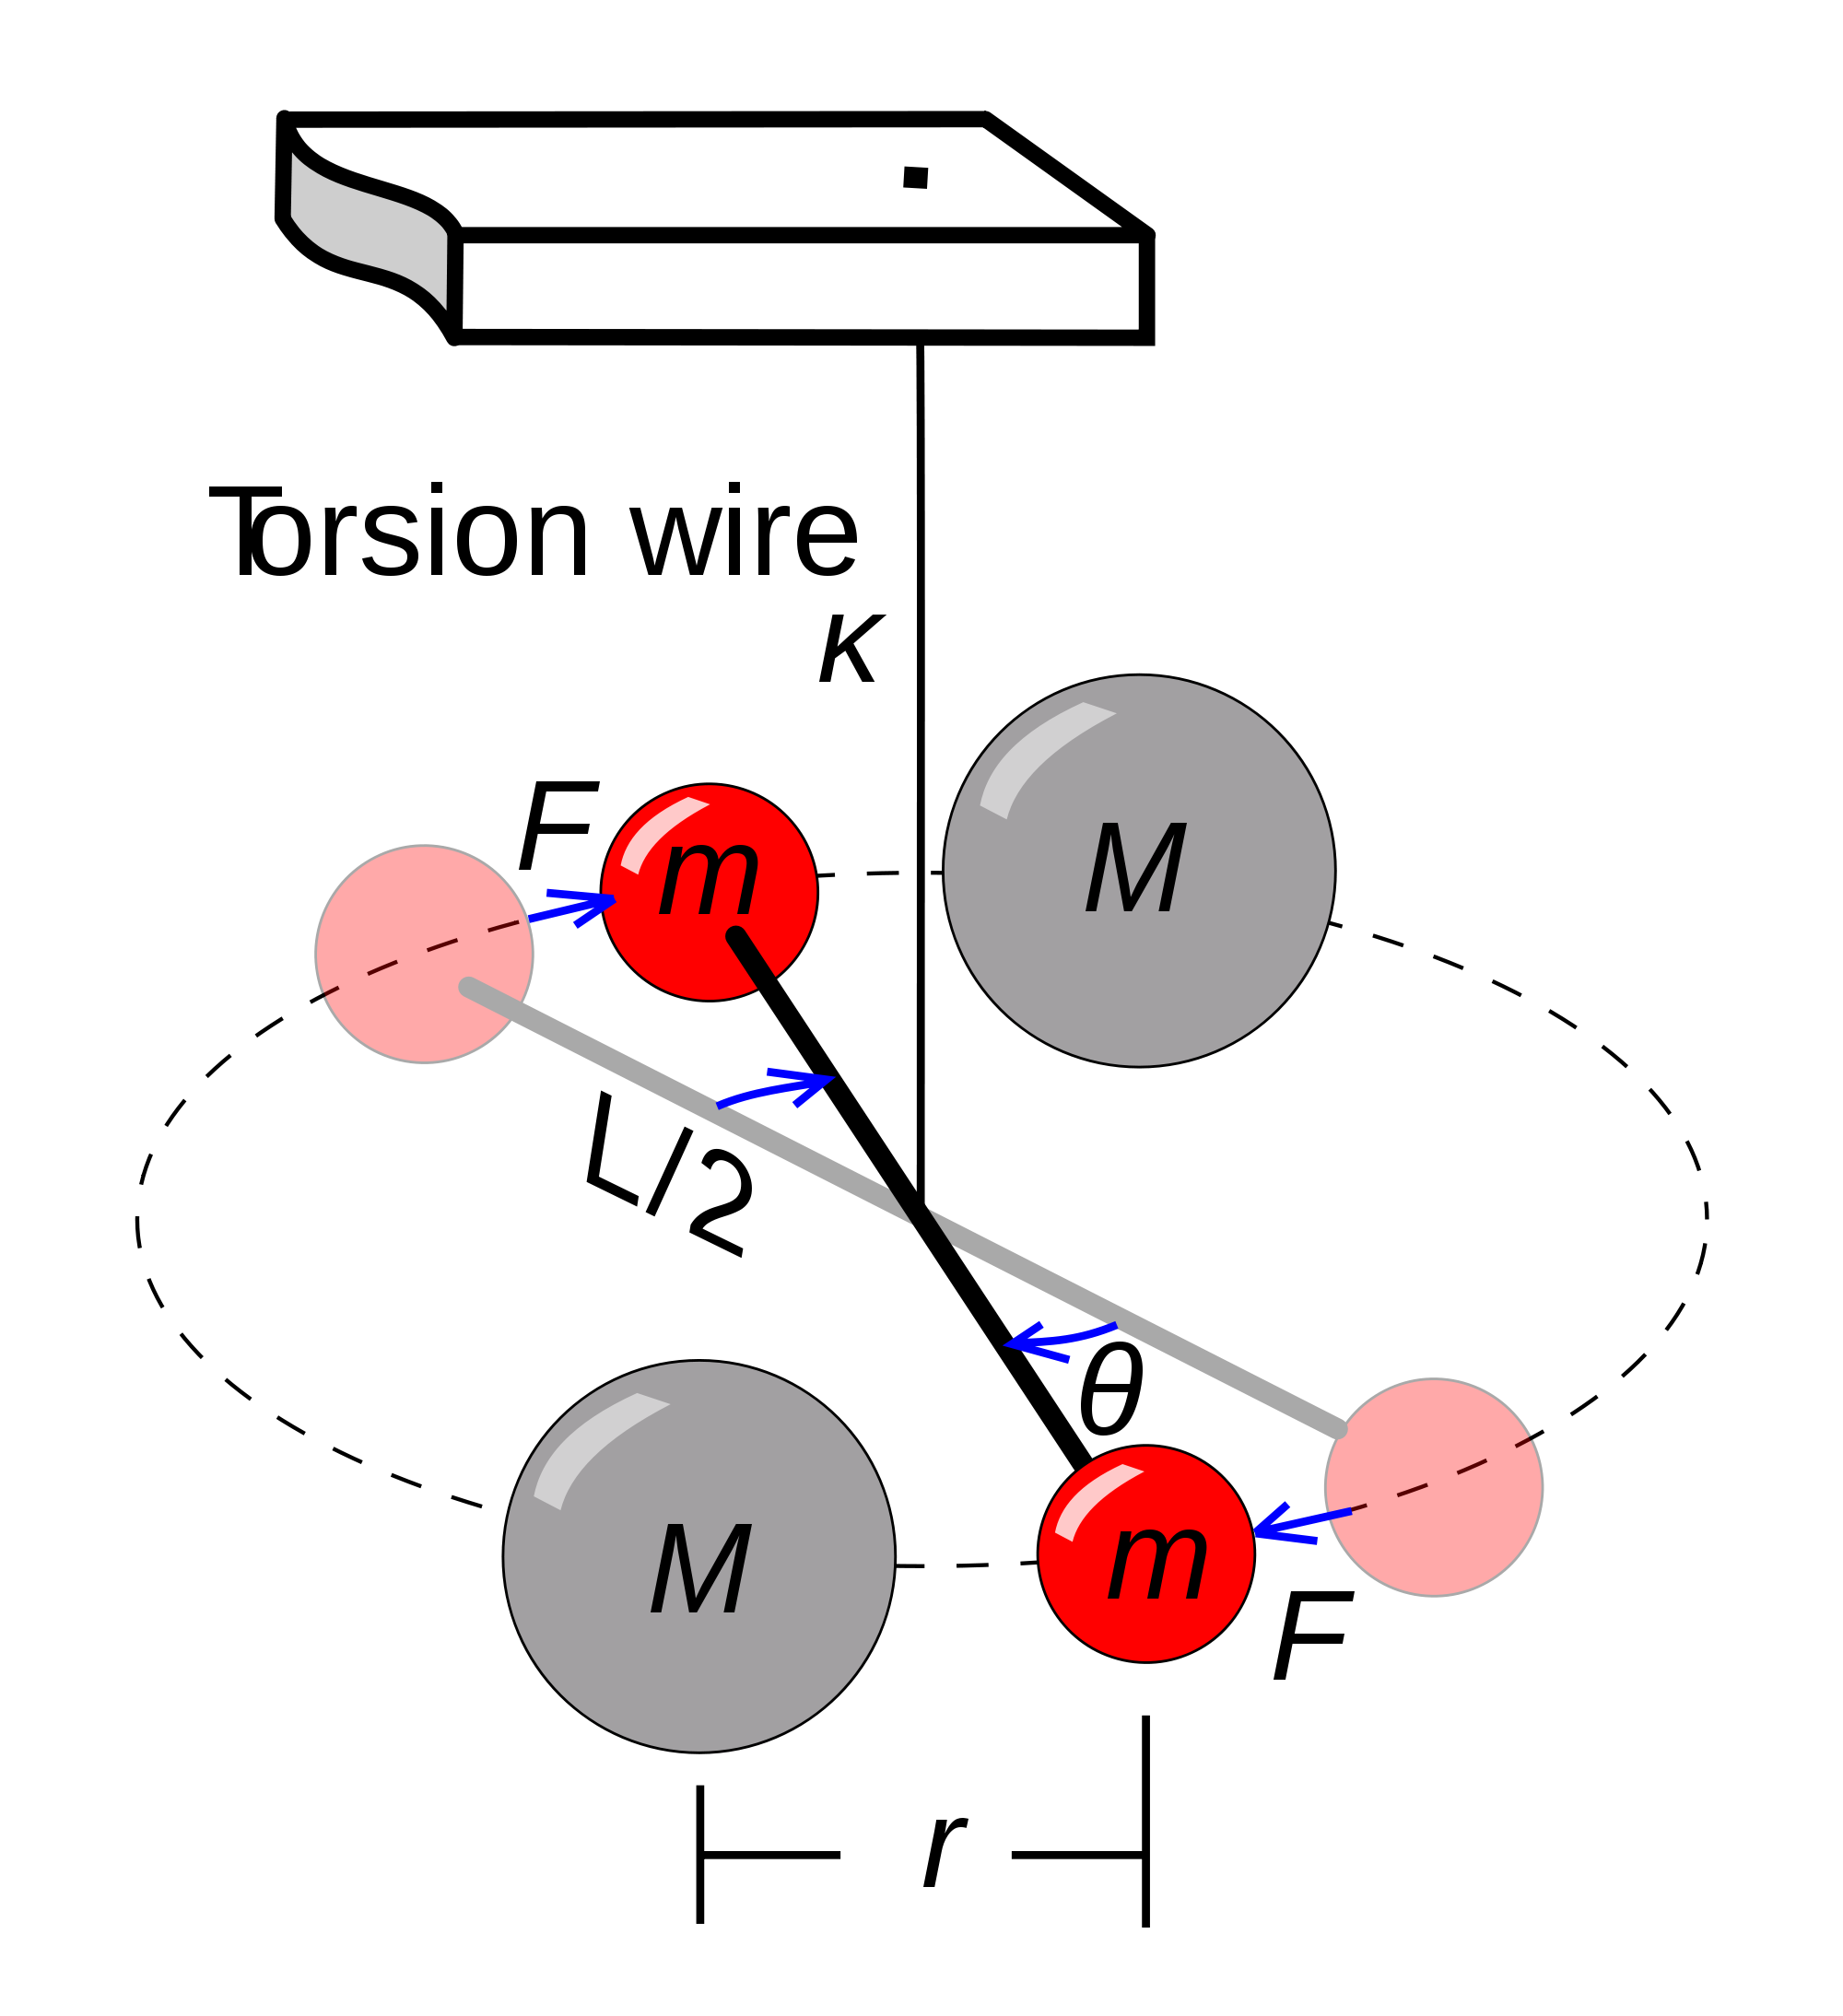
\includegraphics[width=0.5\textwidth]{images/cavendish-torsion-balance.png}
\end{figure}

\exercise{Show that Cavendish also measured density if Earth as a bonus at the same time}

\begin{itemize}
\item Modern $G=6.67384(80)\times 10^{-11} Nm^2kg^{-2}=kg^{-1}m^3 s^{-2}$\\
\item Product GM is known to 1 part in $~10^{10}$ from astrophysics observations
\begin{itemize}
\item[$\Rightarrow$] mass is hard to measure gravitationally
\end{itemize}
\item We need a dimensionless number to characterise strength
\item Newton: $\Phi=\frac{GM}{r}$ (potential)
\item In free fall: $\frac{KE}{mass}$, $v^2 ~ \frac{GM}{r}$
\item We claim gravity is strong is free-fall is relativistic, i.e. $v~c$
\item This is an order of magnitude estimate
\end{itemize}


\subsection{Strong vs. weak gravity}
\begin{itemize}
\item Quasi-Newtonian:
\begin{itemize}
\item characterticstic speed of body in free fall: $v^2\sim \frac{GM}{r}$
\end{itemize}
\item Strong gravity leads to relativistic free fall, i.e. $\frac{GM}{Rc^2}\geq 1$ where M is the total mass and R is th characteristic size
\end{itemize}

\begin{table}
\centering
\begin{tabular}{c|cc} 
 & $\frac{GM}{Rc^2} \lll 1$ & $\frac{GM}{Rc^2}\geq 1$\\
\hline $v \ll c$ & Newtonian & CAN'T EXIST \\
$v\sim c$ & special rel. & full GR (difficult)
\end{tabular}
\end{table}

\example{1.1}{
$M=M_{\odot}$ (mass of the Sun)
\begin{align*}
R & \sim \frac{GM}{c^2} \text{\quad boundary of strong regime}\\
&\sim \frac{10^{-10}10^{30}}{10^{17}}\\
&\sim \text{km}
\end{align*}
cf. Schwarz radius of black hole $=\frac{2GM}{c^2}$
}
\example{1.2}{
Density of black hole with mass of $M_\odot$
\begin{align*}
&\sim \frac{M}{R^3}\sim\frac{10^{30}kg}{(km)^3}\\
&\sim 10^{21}kgm^{-3}
\end{align*}
How does this density compare to maximum density of (say) nuclear matter? Let's compare.
\begin{align*}
\frac{m_n}{(1fm)^3}\sim \frac{10^{-27}kg}{10^{-45}m^3}\sim 10^{18}kgm^{-3}
\end{align*}
We see a black hole is more dense that a nuclei. The characteristic size of a particle $1fm\sim\Delta x\sim \frac{\hbar}{\Delta p}\sim \frac{\hbar}{m_n c}$, due to Heisenberg's uncertainty principle, and also the Pauli exclusion principle.
}
More generally: density of material that froms black hole $\sim\frac{M}{R^3}$, but note $M=\frac{c^2R}{G}$ density $\rho \propto \frac{1}{R^2}$. This means that denser black holes are smaller.

\exercise{Estimate the strength of gravity $\frac{GM}{Rc^2}$ on Earth.}

\example{2}
{
The Universe is composed of 5\% baryons + 25\% dark matter + 70\% dark energy. Estimate M and R.\\
$R\sim \SI{10}{Gpc}$
\begin{itemize}
\item Mass of baryons 
\begin{itemize}
\item $10^{11}$ stars in Milky Way
\item $(10^4)^3$ galaxies in Universe
\item $\Rightarrow M_{\text{baryons}}\sim10^{23}M_\odot\sim 10^{53}kg$
\end{itemize}
\end{itemize} 
\begin{equation}
\frac{GM_tot}{Rc^2}\sim\frac{10^{-10}\dot 10^{53}\dot 10}{10^{27} \dot 10^{17}}\sim 1
\end{equation}
\begin{align*}
\text{Density }\rho\sim\frac{M_{tot}}{R_{tot}^3}&\sim\frac{c^2}{R^2G}\text{, use }\frac{GM}{Rc^2}\sim 1\\
&\sim\frac{1}{G\times(\text{age of universe})^2}
\end{align*}
cf. critical density from Friedmann equations $\rho_{crit}=\frac{3H_0^2}{8\pi G}$.\\
Recall Hubble constant $H_0\sim \frac{1}{\text{age}}$.
}
The critical density is the density of the universe at which expansion will asymptotically slow. Too dense leads to big crunch, too low leads to unbounded expansion.
\exercise{How do we reconcile a ``flat" universe from critical density with the ``curved" universe?}




\pagebreak

%-----------------------------------------
\end{document}







